\addtocontents{toc}{\protect\newpage}
\chapter{Математичні компоненти}

Четвертий розділ надає приклади математичного моделювання
та складних теорем теорії категорій, теорій топосів, теорії гомотопій, тощо.

\section{Теорія категорій}

\subsection{Категорія}

\begin{definition} (Category Signature).
The signature of category is
a $\Sigma_{A:U}A \rightarrow A \rightarrow U$ where $U$ could be any universe.
The $pr_1$ projection is called $Ob$ and $pr_2$ projection is
called $Hom(a,b)$, where $a,b:Ob$.
\begin{lstlisting}
cat: U = (A: U) * (A -> A -> U)
\end{lstlisting}
\end{definition}

Precategory $C$ defined as set of $Hom_C(a,b)$ where $a,b:Ob_C$
are objects defined by its $id$ arrows $Hom_C(x,x)$.
Properfies of left and right units included with composition c
and its associativity.

\begin{definition} (Precategory).
More formal, precategory $C$ consists of the following.
(i) A type $Ob_C$, whose elements are called objects;
(ii) for each $a,b: Ob_C$, a set $Hom_C(a,b)$, whose
elements are called arrows or morphisms.
(iii) For each $a: Ob_C$, a morphism $1_a : Hom_C(a,a)$,
called the identity morphism.
(iv) For each $a,b,c: Ob_C$, a function
$Hom_C(b,c) \rightarrow Hom_C(a,b) \rightarrow Hom_C(a,c)$
called composition, and denoted $g \circ f$.
(v) For each $a,b: Ob_C$ and $f: Hom_C(a,b)$,
$f = 1_b \circ f$ and $f = f \circ 1_a$.
(vi) For each $a,b,c,d: A$ and
$f: Hom_C(a,b)$, $g: Hom_C(b,c)$, $h: Hom_C(c,d)$,
$h \circ (g \circ f ) = (h \circ g) \circ f$.
\end{definition}

\begin{definition} (Small Category).
If for all $a,b: Ob$ the $Hom_C(a,b)$ forms a Set, then
such category is called small category.
\begin{lstlisting}
isPrecategory (C: cat): U
  = (id: (x: C.1) -> C.2 x x)
  * (c: (x y z: C.1) -> C.2 x y -> C.2 y z -> C.2 x z)
  * (homSet: (x y: C.1) -> isSet (C.2 x y))
  * (left: (x y: C.1) -> (f: C.2 x y)
  -> Path (C.2 x y) (c x x y (id x) f) f)
  * (right: (x y: C.1) -> (f: C.2 x y)
  -> Path (C.2 x y) (c x y y f (id y)) f)
  * ( (x y z w: C.1) (f: C.2 x y) (g: C.2 y z)
    (h: C.2 z w) -> Path (C.2 x w)
    (c x z w (c x y z f g) h) (c x y w f (c y z w g h)))
\end{lstlisting}
precategory: U = (C: cat) * isPrecategory C
\begin{lstlisting}
\end{lstlisting}
\end{definition}

Accessors of the precategory structure.
For $Ob$ is carrier and for $Hom$ is hom.

\begin{lstlisting}
carrier (C: precategory): U = C.1.1
hom     (C: precategory) (a b: carrier C): U = C.1.2 a b
path    (C: precategory) (x: carrier C): hom C x x = C.2.1 x
compose (C: precategory) (x y z: carrier C)
        (f: hom C x y) (g: hom C y z): hom C x z = C.2.2.1 x y z f g
\end{lstlisting}

\subsection{(Ко)термінал}
\begin{definition} (Initial Object).
Is such object $Ob_C$, that $\Pi_{x,y:Ob_C}$ $isContr(Hom_C(x,y))$.
\end{definition}

\begin{definition} (Terminal Object).
Is such object $Ob_C$, that $\Pi_{x,y:Ob_C}$ $isContr(Hom_C(y,x))$.
\begin{lstlisting}
isInitial (C: precategory) (x: carrier C): U
  = (y: carrier C) -> isContr (hom C x y)
isTerminal (C: precategory) (y: carrier C): U
  = (x: carrier C) -> isContr (hom C x y)
initial (C: precategory): U
  = (x: carrier C) * isInitial  C x
terminal(C: precategory): U
  = (y: carrier C) * isTerminal C y
\end{lstlisting}
\end{definition}

\subsection{Функтор}
\begin{definition} (Category Functor). Let $A$ and $B$ be precategories.
A functor $F : A \rightarrow B$ consists of: (i) A function $F_{Ob}: Ob_hA \rightarrow Ob_B$;
(ii) for each $a,b:Ob_A$, a function $F_{Hom}:Hom_A(a,b)\rightarrow Hom_B(F_{Ob}(a),F_{Ob}(b))$;
(iii) for each $a:Ob_A$, $F_{Ob}(1_a) = 1_{F_{Ob}}(a)$;
(iv) for $a,b,c:Ob_A$ and $f: Hom_A(a,b)$ and $g: Hom_A(b,c)$, $F(g\circ f) = F_{Hom}(g)\circ F_{Hom}(f)$.
\begin{lstlisting}
catfunctor (A B: precategory): U
  = (ob: carrier A -> carrier B)
  * (mor: (x y: carrier A) -> hom A x y -> hom B (ob x) (ob y))
  * (id: (x: carrier A) -> Path (hom B (ob x) (ob x))
    (mor x x (path A x)) (path B (ob x)))
  * ((x y z: carrier A) -> (f: hom A x y) -> (g: hom A y z) ->
     Path (hom B (ob x) (ob z)) (mor x z (compose A x y z f g))
      (compose B (ob x) (ob y) (ob z) (mor x y f) (mor y z g)))
\end{lstlisting}
\end{definition}

\subsection{Натуральні перетворення}
\begin{definition} (Natural Transformation).
For functors $F,G: C \rightarrow D$,
a nagtural transformation $\gamma: F \rightarrow G$ consists of:
(i) for each $x:C$, a morphism $\gamma_a : Hom_D(F(x),G(x))$;
(ii) for each $x,y:C$ and $f: Hom_C(x,y)$, $G(f)\circ \gamma_x = \gamma_y \circ F(g)$.
\begin{lstlisting}
isNaturalTrans (C D: precategory)
               (F G: catfunctor C D)
               (eta: (x: carrier C) -> hom D (F.1 x) (G.1 x)): U
  = (x y: carrier C) (h: hom C x y) ->
     Path (hom D (F.1 x) (G.1 y))
     (compose D (F.1 x) (F.1 y) (G.1 y) (F.2.1 x y h) (eta y))
     (compose D (F.1 x) (G.1 x) (G.1 y) (eta x) (G.2.1 x y h))

ntrans (C D: precategory) (F G: catfunctor C D): U
  = (eta: (x: carrier C) -> hom D (F.1 x) (G.1 x))
  * (isNaturalTrans C D F G eta)
\end{lstlisting}
\end{definition}

\subsection{Розширення Кана}
\begin{definition} (Kan Extension).
\begin{lstlisting}
extension (C C' D: precategory)
    (K: catfunctor C C') (G: catfunctor C D) : U
  = (F: catfunctor C' D)
  * (ntrans C D (compFunctor C C' D K F) G)
\end{lstlisting}
\end{definition}

\subsection{Ізоморфізм категорій}
\begin{definition} (Category Isomorphism).
A morphism $f : Hom_A(a,b)$ is an iso
if there is a morphism $g: Hom_A(b,a)$ such that
$1_a =_\eta g \circ f$ and
$f \circ g =_\epsilon 1_b = g$. "f is iso" is
a mere proposition.
If A is a precategory and $a,b: A$,
then $a = b \rightarrow iso_A(a,b)$ (idtoiso).
\begin{lstlisting}
iso (C: precategory) (A B: carrier C): U
  = (f: hom C A B)
  * (g: hom C B A)
  * (eta: Path (hom C A A) (compose C A B A f g) (path C A))
  * (Path (hom C B B) (compose C B A B g f) (path C B))
\end{lstlisting}
\end{definition}

\subsection{Резк-поповнення}
\begin{definition} (Category).
A category is a precategory
such that for all $a:Ob_C$, the $\Pi_{A:Ob_C} isContr \Sigma_{B:Ob_C} iso_C(A,B)$.
\begin{lstlisting}
isCategory (C: precategory): U
  = (A: carrier C) -> isContr ((B: carrier C) * iso C A B)
    category: U = (C: precategory) * isCategory C
\end{lstlisting}
\end{definition}

\subsection{Конструкції}

\subsubsection{(Ко)продукти категорій}
\begin{definition} (Category Product).
\begin{lstlisting}
Product    (X Y: precategory) : precategory
Coproduct  (X Y: precategory) : precategory
\end{lstlisting}
\end{definition}

\subsubsection{Обернена категорія}
\begin{definition} (Opposite Category). The opposite category to category $C$
is a category $C^{op}$ with same structure, except all arrows are inverted.
\begin{lstlisting}
opCat (P: precategory): precategory
\end{lstlisting}
\end{definition}

\subsubsection{(Ко)слайс категорія}
\begin{definition} (Slice Category).
\end{definition}
\begin{definition} (Coslice Category).
\begin{lstlisting}
sliceCat (C D: precategory)
    (a: carrier (opCat C))
    (F: catfunctor D (opCat C))
  : precategory
  = cosliceCat (opCat C) D a F

cosliceCat (C D: precategory)
  (a: carrier C)
  (F: catfunctor D C) : precategory
\end{lstlisting}
\end{definition}

\subsubsection{Універсальна властивість}
\begin{definition} (Universal Mapping Property).
\begin{lstlisting}
initArr (C D: precategory)
  (a: carrier C)
  (F: catfunctor D C): U = initial (cosliceCat C D a F)

termArr (C D: precategory)
  (a: carrier (opCat C))
  (F: catfunctor D (opCat C)): U = terminal (sliceCat C D a F)
\end{lstlisting}
\end{definition}

\subsubsection{Одинична категорія}
\begin{definition} (Unit Category).
In unit category both $Ob = \top$ and $Hom = \top$.
\begin{lstlisting}
unitCat: precategory
\end{lstlisting}
\end{definition}

\subsection{Приклади}
\subsubsection{Категорія множин}
\begin{definition} (Category of Sets).
\begin{lstlisting}
Set: precategory = ((Ob,Hom),id,c,HomSet,L,R,Q) where
  Ob: U = SET
  Hom (A B: Ob): U = A.1 -> B.1
  id (A: Ob): Hom A A = idfun A.1
  c (A B C: Ob) (f: Hom A B) (g: Hom B C): Hom A C
   = o A.1 B.1 C.1 g f
  HomSet (A B: Ob): isSet (Hom A B) = setFun A.1 B.1 B.2
  L (A B: Ob) (f: Hom A B): Path (Hom A B) (c A A B (id A) f) f
   = refl (Hom A B) f
  R (A B: Ob) (f: Hom A B): Path (Hom A B) (c A B B f (id B)) f
   = refl (Hom A B) f
  Q (A B C D: Ob) (f: Hom A B) (g: Hom B C) (h: Hom C D)
   : Path (Hom A D) (c A C D (c A B C f g) h) (c A B D f (c B C D g h))
   = refl (Hom A D) (c A B D f (c B C D g h))
\end{lstlisting}
\end{definition}

\subsubsection{Категорія функцій}
\begin{definition} (Category of Functions over Sets).
\begin{lstlisting}
Functions (X Y: U) (Z: isSet Y): precategory
   = ((Ob,Hom),id,c,HomSet,L,R,Q) where
  Ob: U = X -> Y
  Hom (A B: Ob): U = id (X -> Y)
  id (A: Ob): Hom A A = idfun (X -> Y)
  c (A B C: Ob) (f: Hom A B) (g: Hom B C): Hom A C = idfun (X -> Y)
  HomSet (A B: Ob): isSet (Hom A B) = setFun Ob Ob (setFun X Y Z)
  L (A B: Ob) (f: Hom A B): Path (Hom A B) (c A A B (id A) f) f = axiom
  R (A B: Ob) (f: Hom A B): Path (Hom A B) (c A B B f (id B)) f = axiom
  Q (A B C D: Ob) (f: Hom A B) (g: Hom B C) (h: Hom C D)
   : Path (Hom A D) (c A C D (c A B C f g) h)
                    (c A B D f (c B C D g h)) = axiom
\end{lstlisting}
\end{definition}

\subsubsection{Категорія категорій}
\begin{definition} (Category of Categories).
\begin{lstlisting}
Cat: precategory = ((Ob,Hom),id,c,HomSet,L,R,Q) where
  Ob: U = precategory
  Hom (A B: Ob): U = catfunctor A B
  id (A: Ob): catfunctor A A = idFunctor A
  c (A B C: Ob) (f: Hom A B) (g: Hom B C): Hom A C
   = compFunctor A B C f g
  HomSet (A B: Ob): isSet (Hom A B) = axiom
  L (A B: Ob) (f: Hom A B): Path (Hom A B) (c A A B (id A) f) f = axiom
  R (A B: Ob) (f: Hom A B): Path (Hom A B) (c A B B f (id B)) f = axiom
  Q (A B C D: Ob) (f: Hom A B) (g: Hom B C) (h: Hom C D)
   : Path (Hom A D) (c A C D (c A B C f g) h)
                    (c A B D f (c B C D g h)) = axiom
\end{lstlisting}
\end{definition}

\subsubsection{Категорія функторів}
\begin{definition} (Category of Functors).
\begin{lstlisting}
Func (X Y: precategory): precategory
   = ((Ob,Hom),id,c,HomSet,L,R,Q) where
  Ob: U = catfunctor X Y
  Hom (A B: Ob): U = ntrans X Y A B
  id (A: Ob): ntrans X Y A A = axiom
  c (A B C: Ob) (f: Hom A B) (g: Hom B C): Hom A C = axiom
  HomSet (A B: Ob): isSet (Hom A B) = axiom
  L (A B: Ob) (f: Hom A B): Path (Hom A B) (c A A B (id A) f) f = axiom
  R (A B: Ob) (f: Hom A B): Path (Hom A B) (c A B B f (id B)) f = axiom
  Q (A B C D: Ob) (f: Hom A B) (g: Hom B C) (h: Hom C D)
   : Path (Hom A D) (c A C D (c A B C f g) h)
                    (c A B D f (c B C D g h)) = axiom
\end{lstlisting}
\end{definition}

\subsection{k-морфізми}

\begin{definition} ($k$-Morphism).
The k-morphism is defined as morphism
between $(k-1)$-morphism. The base of induction, the $0$-morphism is
defined as object of $1$-category, which is precategory.
\begin{lstlisting}
equiv: U
functor (C D: cat): U
ntrans (C D: cat) (F G: functor C D): U
modification (C D: cat) (F G: functor C D) (I J: ntrans C D F G): U
\end{lstlisting}
І так далі.
\end{definition}

\subsection{2-категорія}
\begin{definition} (2-Category).
\begin{lstlisting}
Cat2 : U
  = (Ob: U)
  * (Hom:  (A B: Ob) -> U)
  * (Hom2: (A B: Ob) -> (C F: Hom A B) -> U)
  * (id:     (A: Ob) -> Hom A A)
  * (id2:    (A: Ob) -> (B: Hom A A) -> Hom2 A A B B)
  * (c:  (A B C: Ob) (f: Hom A B) (g: Hom B C) -> Hom A C)
  * (c2:   (A B: Ob) (X Y Z: Hom A B)
    (f: Hom2 A B X Y) (g: Hom2 A B Y Z) -> Hom2 A B X Z)
\end{lstlisting}
\end{definition}

\subsection{Аддитивна категорія}

%\subsection{Абелева категорія}

\subsection{Група Гротендіка}

\subsection{Категорія Гротендіка}

\section{Теорія топосів}

One can admit two topos theory lineages. One lineage takes its roots from published
by Jean Leray in 1945 initial work on sheaves and spectral sequences. Later this lineage
was developed by Henri Paul Cartan, André Weil. The peak of lineage was settled
with works by Jean-Pierre Serre, Alexander Grothendieck, and Roger Godement.

Second remarkable lineage take its root from William Lawvere and
Myles Tierney. The main contribution is the reformulation of Grothendieck topology
by using subobject classifier.

\begin{definition} (Categorical Pullback).
The pullback of the cospan $A \mapright{f} C \mapleft{g} B$ is a object $A \times_{C} B$ with
morphisms $pb_1 : \times_C \rightarrow A $, $pb_2 : \times_C \rightarrow B$, such that
diagram commutes:
\begin{center}
\begin{tikzpicture}
  \matrix (m) [matrix of math nodes,row sep=3em,column sep=3em,minimum width=2em]
  {
     A \times_{C} B & B \\
     A & C\\};
  \path[-stealth]
    (m-1-1) edge node [above] {$pb_2$} (m-1-2)
            edge node [above] {$$} (m-2-2)
    (m-1-1) edge node [left]  {$f$} (m-2-1)
    (m-1-2) edge node [right] {$pb_1$} (m-2-2)
    (m-2-1) edge node [above] {$g$} (m-2-2);
\end{tikzpicture}
\end{center}
Pullback $(\times_C,pb_1,pb_2)$ must be universal, means for any $(D,q_1,q_2)$
for which diagram also commutes there must exists a unique $u: D \rightarrow \times_C$,
such that $pb_1 \circ u = q_1$ and $pb_2 \circ q_2$.
\begin{lstlisting}
homTo  (C: precategory) (X: carrier C): U
  = (Y: carrier C) * hom C Y X
cospan (C: precategory): U
  = (X: carrier C) * (_: homTo C X) * homTo C X
cospanCone (C: precategory) (D: cospan C): U
  = (W: carrier C) * hasCospanCone C D W
cospanConeHom (C: precategory) (D: cospan C)
    (E1 E2: cospanCone C D) : U
  = (h: hom C E1.1 E2.1) * isCospanConeHom C D E1 E2 h
isPullback (C: precategory) (D: cospan C) (E: cospanCone C D) : U
  = (h: cospanCone C D) -> isContr (cospanConeHom C D h E)
hasPullback (C: precategory) (D: cospan C) : U
  = (E: cospanCone C D) * isPullback C D E
\end{lstlisting}
\end{definition}

\begin{definition} (Category Functor).
Let $A$ and $B$ be precategories.
A functor $F : A \rightarrow B$ consists of: (i) A function $F_{Ob}: Ob_hA \rightarrow Ob_B$;
(ii) for each $a,b:Ob_A$, a function $F_{Hom}:Hom_A(a,b)\rightarrow Hom_B(F_{Ob}(a),F_{Ob}(b))$;
(iii) for each $a:Ob_A$, $F_{Ob}(1_a) = 1_{F_{Ob}}(a)$;
(iv) for $a,b,c:Ob_A$ and $f: Hom_A(a,b)$ and $g: Hom_A(b,c)$, $F(g\circ f) = F_{Hom}(g)\circ F_{Hom}(f)$.
\begin{lstlisting}
catfunctor (A B: precategory): U
  = (ob: carrier A -> carrier B)
  * (mor: (x y:carrier A)->hom A x y->hom B(ob x)(ob y))
  * (id: (x: carrier A) -> Path (hom B (ob x) (ob x))
    (mor x x (path A x)) (path B (ob x)))
  * ((x y z: carrier A) -> (f: hom A x y) -> (g: hom A y z) ->
    Path (hom B (ob x) (ob z)) (mor x z (compose A x y z f g))
         (compose B (ob x) (ob y) (ob z) (mor x y f) (mor y z g)))
\end{lstlisting}
\end{definition}

\begin{definition} (Terminal Object). Is such object $\mathrm{Ob}_C$,
that
$$
    \prod_{x,y:\mathrm{Ob}_C} \mathrm{isContr} (\mathrm{Hom}_C(y,x)).
$$
\begin{lstlisting}
isTerminal (C: precategory) (y: carrier C): U
  = (x: carrier C) -> isContr (hom C x y)
terminal (C: precategory): U
  = (y: carrier C) * isTerminal C y
\end{lstlisting}
\end{definition}

%\begin{definition}
%\begin{lstlisting}
%\end{lstlisting}
%\end{definition}

\subsection{Теорія множин}

Here is given the $\infty$-groupoid model of sets.

\begin{definition} (Mere proposition, $\mathrm{PROP}$).
A type P is a mere proposition if for all $x,y: P$ we have $x=y$:
$$
    \mathrm{isProp}(P) = \prod_{x,y:P}(x=y).
$$
\end{definition}

\begin{definition} (0-type).
A type A is a 0-type is for all $x,y: A$ and $p,q: x =_A y$ we have $p = q$.
\end{definition}

\begin{definition} (1-type).
A type A is a 1-type if for all $x,y: A$ and $p,q: x =_A y$ and $r,s:p =_{=_A} q$, we have $r = s$.
\end{definition}

\begin{definition} (A set of elements, $\mathrm{SET}$).
A type A is a $\mathrm{SET}$ if for all $x,y: A$ and $p,q: x = y$, we have $p = q$:
$$
    \mathrm{isSet}(A) = \prod_{x,y:A}\prod_{p,q:x=y}(p=q).
$$
\end{definition}

\begin{definition}
\begin{lstlisting}
data N = Z  | S (n: N)

n_grpd (A: U) (n: N): U = (a b: A) -> rec A a b n where
  rec (A: U) (a b: A) : (k: N) -> U
    = split { Z -> Path A a b ; S n -> n_grpd (Path A a b) n }

isContr (A: U): U = (x: A) * ((y: A) -> Path A x y)
isProp  (A: U): U = n_grpd A Z
isSet   (A: U): U = n_grpd A (S Z)
PROP  : U = (X:U) * isProp X
SET   : U = (X:U) * isSet X
\end{lstlisting}
\end{definition}

\begin{definition} ($\Pi$-Contractability).
If fiber is set thene path space between any sections is contractible.
\begin{lstlisting}
setPi (A: U) (B: A -> U) (h: (x: A) -> isSet (B x)) (f g: Pi A B)
      (p q: Path (Pi A B) f g)
    : Path (Path (Pi A B) f g) p q
\end{lstlisting}
\end{definition}

\begin{definition} ($\Sigma$-Contractability).
If fiber is set then $\Sigma$ is set.
\begin{lstlisting}
setSig (A:U) (B: A -> U) (base: isSet A)
       (fiber: (x:A) -> isSet (B x)) : isSet (Sigma A B)
\end{lstlisting}
\end{definition}

\begin{definition} (Unit type, $1$).
The unit $1$ is a type with one element.
\begin{lstlisting}
data unit = tt
unitRec (C: U) (x: C): unit -> C = split tt -> x
unitInd (C: unit -> U) (x: C tt): (z:unit) -> C z
  = split tt -> x
\end{lstlisting}
\end{definition}

\begin{theorem} (Category of Sets, $\mathbf{Set}$).
Sets forms a Category.
All compositional theorems proved by using reflection rule of internal language.
The proof that $\mathrm{Hom}$ forms a set is taken through $\Pi$-contractability.
\begin{lstlisting}
Set: precategory = ((Ob,Hom),id,c,HomSet,L,R,Q) where
  Ob: U = SET
  Hom (A B: Ob): U = A.1 -> B.1
  id (A: Ob): Hom A A = idfun A.1
  c (A B C: Ob) (f: Hom A B) (g: Hom B C): Hom A C
    = o A.1 B.1 C.1 g f
  HomSet (A B: Ob): isSet (Hom A B) = setFun A.1 B.1 B.2
  L (A B:Ob) (f:Hom A B): Path (Hom A B)(c A A B (id A)f)f
    = refl (Hom A B) f
  R (A B:Ob) (f:Hom A B): Path (Hom A B)(c A B B f(id B))f
    = refl (Hom A B) f
  Q (A B C D: Ob) (f:Hom A B) (g:Hom B C) (h:Hom C D)
    : Path (Hom A D) (c A C D (c A B C f g) h)
                     (c A B D f (c B C D g h))
    = refl (Hom A D) (c A B D f (c B C D g h))
\end{lstlisting}
\end{theorem}

Topos theory extends category theory with notion of topological
structure but reformulated in a categorical way
as a category of sheaves on a site or as one that has cartesian closure
and subobject classifier. We give here two definitions.

\subsection{Топологічна структура}

\begin{definition} (Topology). The topological structure on $\mathrm{A}$
(or topology) is a subset $S \in \mathrm{A}$ with following properties:
i) any finite union of subsets of $\mathrm{S}$ is belong to $\mathrm{S}$;
ii) any finite intersection of subsets of $\mathrm{S}$ is belong to $\mathrm{S}$.
Subets of $\mathrm{S}$ are called open sets of family $\mathrm{S}$.
\begin{lstlisting}
Structure topology (A : Type) := {
          open :> (A -> Prop) -> Prop;
          empty_open: open (empty _);
          full_open:  open (full _);
          inter_open: forall u,
                      open u -> forall v, open v
                             -> open (inter A u v) ;
          union_open: forall s, (subset _ s open)
                             -> open (union A s) }.
\end{lstlisting}
For fully functional general topology theorems and Zorn lemma you can refer to
the Coq library \footnote{https://github.com/verimath/topology}{topology} by Daniel Schepler.
\end{definition}

\subsection{Топос Гротендіка}

Grothendieck Topology is a calculus of coverings which generalizes the algebra
of open covers of a topological space, and can exist on much more general categories.
There are three variants of Grothendieck topology definition:
i) sieves; ii) coverage; iii) covering families.
A category have one of these three is called a Grothendieck site.

{\bf Examples}: Zariski, flat, étale, Nisnevich topologies.

A sheaf is a presheaf (functor from opposite category to category of sets) which
satisties patching conditions arising from Grothendieck topology, and applying
the associated sheaf functor to preashef forces compliance with these conditions.

The notion of Grothendieck topos is a geometric flavour of topos theory,
where topos is defined as category of sheaves on a Grothendieck site with
geometric moriphisms as adjoint pairs of functors between topoi, that
satisfy exactness properties. \cite{Jardine15}

As this flavour of topos theory uses category of sets as a prerequisite,
the formal construction of set topos is cricual in doing sheaf topos theory.

\begin{definition} (Sieves).
Sieves are a family of subfunctors
$$\def\mapright#1{\xrightarrow{{#1}}}
  \def\mapdown#1{\Big\downarrow\rlap{\raise2pt{\scriptstyle{#1}}}}
  \def\mapdiagl#1{\vcenter{\searrow}\rlap{\raise2pt{\scriptstyle{#1}}}}
  \def\mapdiagr#1{\vcenter{\swarrow}\rlap{\raise2pt{\scriptstyle{#1}}}}
  R \subset Hom_C(\_,U), U \in \mathrm{C},
$$
such that following axioms hold: i) (base change) If $R \subset Hom_C(\_,U)$ is covering
and $\phi : V \rightarrow U$ is a morphism of $\mathrm{C}$, then the subfuntor
$$
   \phi^{-1}(R) = \{ \gamma : W \rightarrow V \| \phi \cdot \gamma \in R \}
$$
is covering for $V$; ii) (local character) Suppose that $R,R' \subset Hom_C(\_,U)$ are
subfunctors and R is covering. If $\phi^{-1}(R')$ is covering for
all $\phi : V \rightarrow U$ in $R$, then $R'$ is covering; iii)
$Hom_C(\_,U)$ is covering for all $U \in \mathrm{C}$.
\end{definition}

\begin{definition} (Coverage).
A coverage is a function assigning
to each $\mathrm{Ob}_C$ the family of morphisms $\{f_i : U_i \rightarrow U \}_{i\in I}$ called
covering families, such that for any $g: V \rightarrow U$ exist
a covering family $\{h:V_j \rightarrow V\}_{j \in J}$ such that
each composite $h_j \circ g$ factors some $f_i$:
\begin{tikzcd}
 & V_j \arrow[r, "k"] \arrow[d, "h"]
 & U_i \arrow[d, "f_i"] \\
 & V \arrow[r, "g"] & U
\end{tikzcd}
\begin{lstlisting}
Co (C: precategory) (cod: carrier C) : U
  = (dom: carrier C)
  * (hom C dom cod)

Delta (C: precategory) (d: carrier C) : U
  = (index: U)
  * (index -> Co C d)

Coverage (C: precategory): U
  = (cod: carrier C)
  * (fam: Delta C cod)
  * (coverings: carrier C -> Delta C cod -> U)
  * (coverings cod fam)
\end{lstlisting}
\end{definition}

\begin{definition} (Grothendieck Topology).
Suppose category $\mathrm{C}$ has all pullbacks.
Since $\mathrm{C}$ is small, a pretopology on $\mathrm{C}$ consists of families of sets of
morphisms
$$
    \{ \phi_\alpha : U_\alpha \rightarrow U \}, U \in \mathrm{C},
$$
called covering families, such that following axioms hold:
i) suppose that $\phi_\alpha : U_\alpha \rightarrow U$ is a covering family
and that $\psi : V \rightarrow U$ is a morphism of $\mathrm{C}$.
Then the collection $V \times_U U_\alpha \rightarrow V$ is a cvering family for $V$.
ii) If $\{\phi_\alpha : U_\alpha \rightarrow U \}$ is covering,
and $\{\gamma_{\alpha,\beta} : W_{\alpha,\beta} \rightarrow U_\alpha \}$
is covering for all $\alpha$, then the family of composites
$$
    W_{\alpha,\beta} \mapright{\gamma_{\alpha,\beta}} U_\alpha \mapright{\phi_\alpha} U
$$
is covering; iii) The family $\{1: U \rightarrow U\}$ is covering for all $U \in \mathrm{C}$.
\end{definition}

\begin{definition} (Site).
Site is a category having either a coverage, grothendieck topology, or sieves.
\begin{lstlisting}
site (C: precategory): U
  = (C: precategory) * Coverage C
\end{lstlisting}
\end{definition}

\begin{definition} (Presheaf).
Presheaf of a category $\mathrm{C}$ is a functor from opposite category to category of sets:
$\mathrm{C}^{op} \rightarrow \mathrm{Set}$.
\begin{lstlisting}
presheaf (C: precategory): U
  = catfunctor (opCat C) Set
\end{lstlisting}
\end{definition}

\begin{definition} (Presheaf Category, {\bf PSh}).
Presheaf category {\bf PSh} for a site $\mathrm{C}$ is category
were objects are presheaves and morphisms are natural transformations
of presheaf functors.
\end{definition}

\begin{definition} (Sheaf). Sheaf is a presheaf on a site. In other words
a presheaf $F : \mathrm{C}^{op} \rightarrow \mathbf{Set}$ such that the
cannonical map of inverse limit
$$
    F(U) \rightarrow \lim^{\leftarrow}_{V \to U \in R}{F(V)}
$$
is an isomorphism for each covering sieve $R \subset Hom_C(\_,U)$.
Equivalently, all induced functions
$$
    Hom_C(Hom_C(\_,U),F) \rightarrow Hom_C(R,F)
$$
should be bejections.
\begin{lstlisting}
sheaf (C: precategory): U
  = (S: site C)
  * presheaf S.1
\end{lstlisting}
\end{definition}

\begin{definition} (Sheaf Category, {\bf Sh}).
Sheaf category {\bf Sh}
is a category where objects are sheaves and morphisms are
natural transformation of sheves. Sheaf category is a full subcategory
of category of presheaves {\bf PSh}.
\end{definition}

\begin{definition} (Grothendieck Topos).
Topos is the category of sheaves {\bf Sh}$(C,J)$ on a site $\mathrm{C}$ with topology $J$.
\end{definition}

\begin{theorem} (Giraud).
A category $\mathrm{C}$ is a Grothiendieck topos iff it has following properties:
i) has all finite limits;
ii) has small disjoint coproducts stable under pullbacks;
iii) any epimorphism is coequalizer;
iv) any equivalence relation $R \rightarrow E$ is a kernel pair and has a quotient;
v) any coequalizer $R \rightarrow E \rightarrow Q$ is stably exact;
vi) there is a set of objects that generates $\mathrm{C}$.
\end{theorem}

\begin{definition} (Geometric Morphism). Suppose that $\mathrm{C}$ and $\mathrm{D}$
are Grothendieck sites. A geometric morphism
$$
    f : {\bf Sh}(C) \rightarrow {\bf Sh}(D)
$$
consist of functors $f_* : {\bf Sh}(C) \rightarrow {\bf Sh}(D)$ and
$f^* : {\bf Sh}(D) \rightarrow {\bf Sh}(C)$ such that $f^*$ is
left adjoint to $f_*$ and $f^*$ preserves finite limits. The left adjoint $f^*$ is called
the inverse image functor, while $f_*$ is called the direct image. The inverse image functor
$f^*$ is left and right exact in the sense that it preserves all finite
colimits and limits, respectively.
\end{definition}

\begin{definition} (Cohesive Topos). A topos $E$ is a cohesive topos over a base topos $S$,
if there is a geometric morphism $(p^*,p_*): E \rightarrow S$, such that:
i) exists adjunction $p^! \vdash p_*$ and $ p^! \dashv p_*$;
ii) $p^*$ and $p^!$ are full faithful; iii) $p_!$ preserves finite products.
This quadruple defines adjoint triple:
$$
\int \dashv \fl \dashv \sharp
$$
\end{definition}

\subsection{Елементарний топос}

Giraud theorem was a synonymical topos definition involved only topos
properties but not a site properties. That was step forward on
predicative definition. The other step was made by Lawvere and Tierney,
by removing explicit dependance on categorical model of set
theory (as category of set is used in definition of presheaf). This information
was hidden into subobject classifier which was well defined through
categorical pullback and property of being cartesian
closed (having lambda calculus as internal language).

Elementary topos doesn't involve 2-categorical modeling, so we can construct
set topos without using functors and natural transformations
(what we need in geometrical topos theory flavour). This flavour of topos
theory more suited for logic needs rather that geometry, as its set properties
are hidden under the predicative predicative pullback definition of subobject classifier
rather that functorial notation of presheaf functor. So we can simplify proofs
at the homotopy levels, not to lift everything to 2-categorical model.

\begin{definition} (Monomorphism).
An morphism $f : Y \rightarrow Z $ is a monic or mono
if for any object $X$ and every pair of parralel morphisms $g_1,g_2: X \rightarrow Y$ the
$$
    f \circ g_1 = f \circ g_2 \rightarrow g_1 = g_2.
$$
More abstractly, f is mono if for any $X$ the $\mathrm{Hom}(X,\_)$ takes it to an injective
function between hom sets $\mathrm{Hom}(X,Y) \rightarrow \mathrm{Hom}(X,Z)$.
\begin{lstlisting}
mono (P: precategory) (Y Z: carrier P) (f: hom P Y Z): U
   = (X: carrier P) (g1 g2: hom P X Y)
  -> Path (hom P X Z) (compose P X Y Z g1 f)
                      (compose P X Y Z g2 f)
  -> Path (hom P X Y) g1 g2
\end{lstlisting}
\end{definition}

\begin{definition} (Subobject Classifier\cite{Johnstone14}).
In category $\mathrm{C}$ with finite limits,
a subobject classifier is a monomorphism $true: 1 \rightarrow \Omega$ out of terminal
object $\mathrm{1}$, such that for any mono $U \rightarrow X$ there is a unique
morphism $\chi_U : X \rightarrow \Omega$ and pullback diagram:
\begin{tikzcd}
 & U \arrow[r, "k"] \arrow[d, ""]
 & 1 \arrow[d, "true"] \\
 & X \Omega \arrow[r, "\chi_U"] & \Omega
\end{tikzcd}
\begin{lstlisting}
subobjectClassifier (C: precategory): U
  = (omega: carrier C)
  * (end: terminal C)
  * (trueHom: hom C end.1 omega)
  * (chi: (V X: carrier C) (j: hom C V X) -> hom C X omega)
  * (square: (V X: carrier C) (j: hom C V X) -> mono C V X j
    -> hasPullback C (omega,(end.1,trueHom),(X,chi V X j)))
  * ((V X: carrier C) (j: hom C V X) (k: hom C X omega)
    -> mono C V X j
    -> hasPullback C (omega,(end.1,trueHom),(X,k))
    -> Path (hom C X omega) (chi V X j) k)
\end{lstlisting}
\end{definition}

\begin{theorem} (Category of Sets has Subobject Classifier).
\end{theorem}

\begin{definition} (Cartesian Closed Categories).
The category $\mathrm{C}$ is called cartesian closed if exists all:
i) terminals; ii) products; iii) exponentials. Note that this definition
lacks beta and eta rules which could be found in embedding $\mathbf{MLTT}$.
\begin{lstlisting}
isCCC (C: precategory): U
  = (Exp:   (A B: carrier C) -> carrier C)
  * (Prod:  (A B: carrier C) -> carrier C)
  * (Apply: (A B: carrier C) -> hom C (Prod (Exp A B) A) B)
  * (P1:    (A B: carrier C) -> hom C (Prod A B) A)
  * (P2:    (A B: carrier C) -> hom C (Prod A B) B)
  * (Term:  terminal C)
  * unit
\end{lstlisting}
\end{definition}

\begin{theorem} (Category of Sets is cartesian closed).
As you can see from exp and pro we internalize $\Pi$ and $\Sigma$ types as $\mathrm{SET}$ instances,
the $\mathrm{isSet}$ predicates are provided with contractability.
Exitense of terminals is proved by $\mathrm{propPi}$. The same technique you
can find in $\mathbf{MLTT}$ embedding.
\begin{lstlisting}
cartesianClosure : isCCC Set
  = (expo,prod,appli,proj1,proj2,term,tt) where
    exp (A B: SET): SET = (A.1   -> B.1, setFun A.1 B.1 B.2)
    pro (A B: SET): SET = (prod A.1 B.1, setSig A.1 (\(_ : A.1)
                          -> B.1) A.2 (\(_ : A.1) -> B.2))
    expo:  (A B: SET) -> SET = \(A B: SET) -> exp A B
    prod:  (A B: SET) -> SET = \(A B: SET) -> pro A B
    appli: (A B: SET) -> hom Set (pro (exp A B) A) B
        = \(A B: SET) -> \(x:(pro(exp A B)A).1)-> x.1 x.2
    proj1: (A B: SET) -> hom Set (pro A B) A
        = \(A B: SET) (x: (pro A B).1) -> x.1
    proj2: (A B: SET) -> hom Set (pro A B) B
        = \(A B: SET) (x: (pro A B).1) -> x.2
    unitContr (x: SET) (f: x.1 -> unit) : isContr (x.1 -> unit)
      = (f, \(z: x.1 -> unit) -> propPi x.1 (\(_:x.1)->unit)
           (\(x:x.1) -> propUnit) f z)
    term: terminal Set = ((unit,setUnit),
           \(x: SET) -> unitContr x (\(z: x.1) -> tt))
\end{lstlisting}
Note that rules of cartesian closure forms a type theoretical langage
called lambda calculus.
\end{theorem}

\begin{definition} (Elementary Topos).
Topos is a precategory which is cartesian closed and has subobject classifier.
\begin{lstlisting}
Topos (cat: precategory) : U
  = (cartesianClosure: isCCC cat)
  * subobjectClassifier cat
\end{lstlisting}
\end{definition}

\begin{theorem} (Topos Definitions).
Any Grothendieck topos is an elementary topos too.
The proof is sligthly based on results of Giraud theorem.
\end{theorem}

\begin{theorem} (Category of Sets forms a Topos).
There is a cartesian closure and subobject classifier for a categoty of sets.
\begin{lstlisting}
internal : Topos Set
         = (cartesianClosure,hasSubobject)
\end{lstlisting}
\end{theorem}

\begin{theorem} (Freyd). Main theorem of topos theory\cite{Goldblatt14}.
For any topos $C$ and any $b : \mathrm{Ob}_C$ relative category $C\downarrow b$ is also a topos.
And for any arrow $f: a \rightarrow b$ inverse image functor $f^*: C\downarrow b \rightarrow c\downarrow a$
has left adjoint $\sum_f$ and right adjoin $\prod_f$.
\end{theorem}

\subsection{Висновки}

We gave here constructive definition of topology as finite unions and
intersections of open subsets. Then make this definition categorically
compatible by introducing Grothendieck topology in three different forms: sieves, coverage,
and covering families. Then we defined an elementary topos and introduce category of sets,
and proved that {\bf Set} is cartesian closed, has object classifier and thus a topos.

This intro could be considered as a formal introduction to topos theory (at least of the level of first chapter)
and you may evolve this library to your needs or ask to help porting or developing your application
of topos theory to a particular formal construction.

\section{Алгебраїчна топологія}
\subsection{Теорія груп}
\subsection{Простори}
\subsubsection{Cімпліціальні}
\subsubsection{CW-комплекси}

The definition of homotopy groups, a special role is played
by the inclusions $S^{n-1} \incmap D^n$. We study spaces
obtained iterated attachments of $D^n$ along $S^{n-1}$.

\begin{definition} (Attachment).
Attaching n-cell to a space $X$
along a map $f : S^{n-1} \rightarrow X$ means taking a pushout figure.
$$
\begin{tikzcd}
 & S^{n-1} \arrow[r, "k"] \arrow[d, ""]
 & X \arrow[d, ""] \\
 & D^n \arrow[r, "g"] & \cup_f D^n
\end{tikzcd}
$$
where the notation $X \cup_f D^n$ means result depends
on homotopy class of $f$.
\end{definition}

\begin{definition} (CW-Complex).
Inductively. The only CW-complex of dimention $-1$ is $\varnothing$.
A CW-complex of dimension $\leqslant n$ on $X$ is a
space $X$ obtained by attaching a collection of n-cells
to a CW-complex of dimension $n-1$.

A CW-complex is a space $X$ which is the $colimit(X_i)$ of a
sequence $X_{-1} = \varnothing \incmap X_0 \incmap X_1 \incmap X_2 \incmap ... X$ of
CW-complexes $X_i$ of dimension $\leqslant n$, with $X_{i+1}$
obtained from $X_i$ by i-cell attachments.
Thus if X is a CW-complex, it comes with a filtration
$$
    \varnothing \incmap X_0 \incmap X_1 \incmap X_2 \incmap ... X
$$
where $X_i$ is a CW-complex of dimension $\leqslant i$ called
the i-skeleton, and hence the filtration is called the skeletal
filtration.
\end{definition}

\subsection{Теорія гомотопій}

\subsubsection{Простори петель}

\begin{definition} (Pointed Space). A pointed type $(A,a)$ is a type $A:U$
together with a point $a:A$, called its basepoint.
\begin{lstlisting}
pointed: U = (A: U) * A
point (A: pointed): A.1 = A.2
space (A: pointed): U = A.1
\end{lstlisting}
\end{definition}

\begin{definition} (Loop Space).
$$\Omega(A,a) =_{def} ((a =_A a), refl_A(a)).$$
\begin{lstlisting}
omega1 (A: pointed) : pointed
  = (Path (space A) (point A) (point A), refl A.1 (point A))
\end{lstlisting}
\end{definition}

\begin{definition} (n-Loop Space).
$$
\begin{cases}
\Omega^0(A, a) =_{def} (A, a)\\
\Omega^{n+1}(A,a) =_{def} \Omega^{n}(\Omega(A,a))\\
\end{cases}
$$
\begin{lstlisting}
omega : nat -> pointed -> pointed = split
  zero -> idfun pointed
  succ n -> \(A: pointed) -> omega n (omega1 A)
\end{lstlisting}
\end{definition}

\subsubsection{Обчислення гомотопічних груп}

\begin{definition} (n-th Homotopy Group of m-Sphere).
$$\pi_{n}S^{m} = ||\Omega^{n}(S^{m})||_0.$$
\begin{lstlisting}
piS (n: nat): (m: nat) -> U = split
   zero   -> sTrunc (space (omega n (bool,false)))
   succ x -> sTrunc (space (omega n (Sn (succ x),north)))
\end{lstlisting}
\end{definition}

\begin{theorem} ($\Omega(S^1)=\mathbb{Z}$).
\begin{lstlisting}
data S1 = base
        | loop <i> [ (i=0) -> base ,
                     (i=1) -> base ]

loopS1 : U = Path S1 base base

encode (x:S1) (p:Path S1 base x)
  : helix x
  = subst S1 helix base x p zeroZ

decode : (x:S1) -> helix x -> Path S1 base x = split
  base -> loopIt
  loop @ i -> rem @ i where
    p : Path U (Z -> loopS1) (Z -> loopS1)
      = <j> helix (loop1@j) -> Path S1 base (loop1@j)
    rem : PathP p loopIt loopIt
      = corFib1 S1 helix (\(x:S1)->Path S1 base x) base
        loopIt loopIt loop1 (\(n:Z) ->
        comp (<i> Path loopS1 (oneTurn (loopIt n))
             (loopIt (testIsoPath Z Z sucZ predZ
                      sucpredZ predsucZ n @ i)))
             (<i>(lem1It n)@-i) [])

loopS1eqZ : Path U Z loopS1
  = isoPath Z loopS1 (decode base) (encode base)
    sectionZ retractZ
\end{lstlisting}
\end{theorem}

\subsubsection{Розшарування Хопфа}

This article defines the Hopf Fibration (HF), the concept
of splitting the $S^3$ sphere onto the twisted cartesian product
of spheres $S^1$ and $S^2$.
Basic HF applications are:
1) HF is a Fiber Bundle structure of Dirac Monopole;
2) HF is a map from the $S^3$ in H to the Bloch sphere;
3) If HF is a vector field in $R^3$ then there exists a solution
to compressible non-viscous Navier-Stokes equations.
It was figured out that there are only
4 dimensions of fibers with Hopf invariant 1, namely
$S^0$, $S^1$, $S^3$, $S^7$.

This article consists of two parts:
1) geometric visualization of projection of $S^3$ to $S^2$ (frontend);
2) formal topological version of HF in cubical type theory (backend).
Consider this a basic intro and a summary of results or companion
guide to the chapter 8.5 from HoTT.

\subsubsection*{Геометрична інтерпретація}

Let's imagine $S^3$ as smooth differentiable manifold and build
a projection onto the display as if demoscene is still alive.

\begin{definition} (Sphere $S^3$).
Like a little baby in $\mathbb{R}^4$:
$$
S^3 = \{ (x_0,x_1,x_2,x_3) \in \mathbb{R}^4 : \sum_{i=0}^3 x_i^2 = 1 \};
$$
\end{definition}

after math classes in quaternions $\mathbb{H}$:

$$
S^3 = \{ x \in \mathbb{H} : \|x\| = 1 \}.
$$

\begin{definition} (Locus).
The $S^3$ is realized as a disjoint
union of circular fibers in Hopf coordinates $(\eta,\theta_1,\theta_2)$:
$$
\begin{cases}
x_0 = cos(\theta_1)sin(\eta), \\
x_1 = sin(\theta_1)sin(\eta), \\
x_2 = cos(\theta_2)cos(\eta), \\
x_3 = sin(\theta_2)cos(\eta). \\
\end{cases}
$$
Where $\eta \in [0,\frac{\pi}{2}]$ and $\theta_{1,2} \in [0,2\pi]$.
\end{definition}

\begin{definition} (Mapping on $S^2$).
A mapping of the Locus to the $S^2$ has points on the circles
parametrized by $\theta_2$:
$$
\begin{cases}
x = sin(2\eta)cos(\theta_1), \\
y = sin(2\eta)sin(\theta_1), \\
z = cos(2\eta).
\end{cases}
$$
\begin{figure}
  \centerline{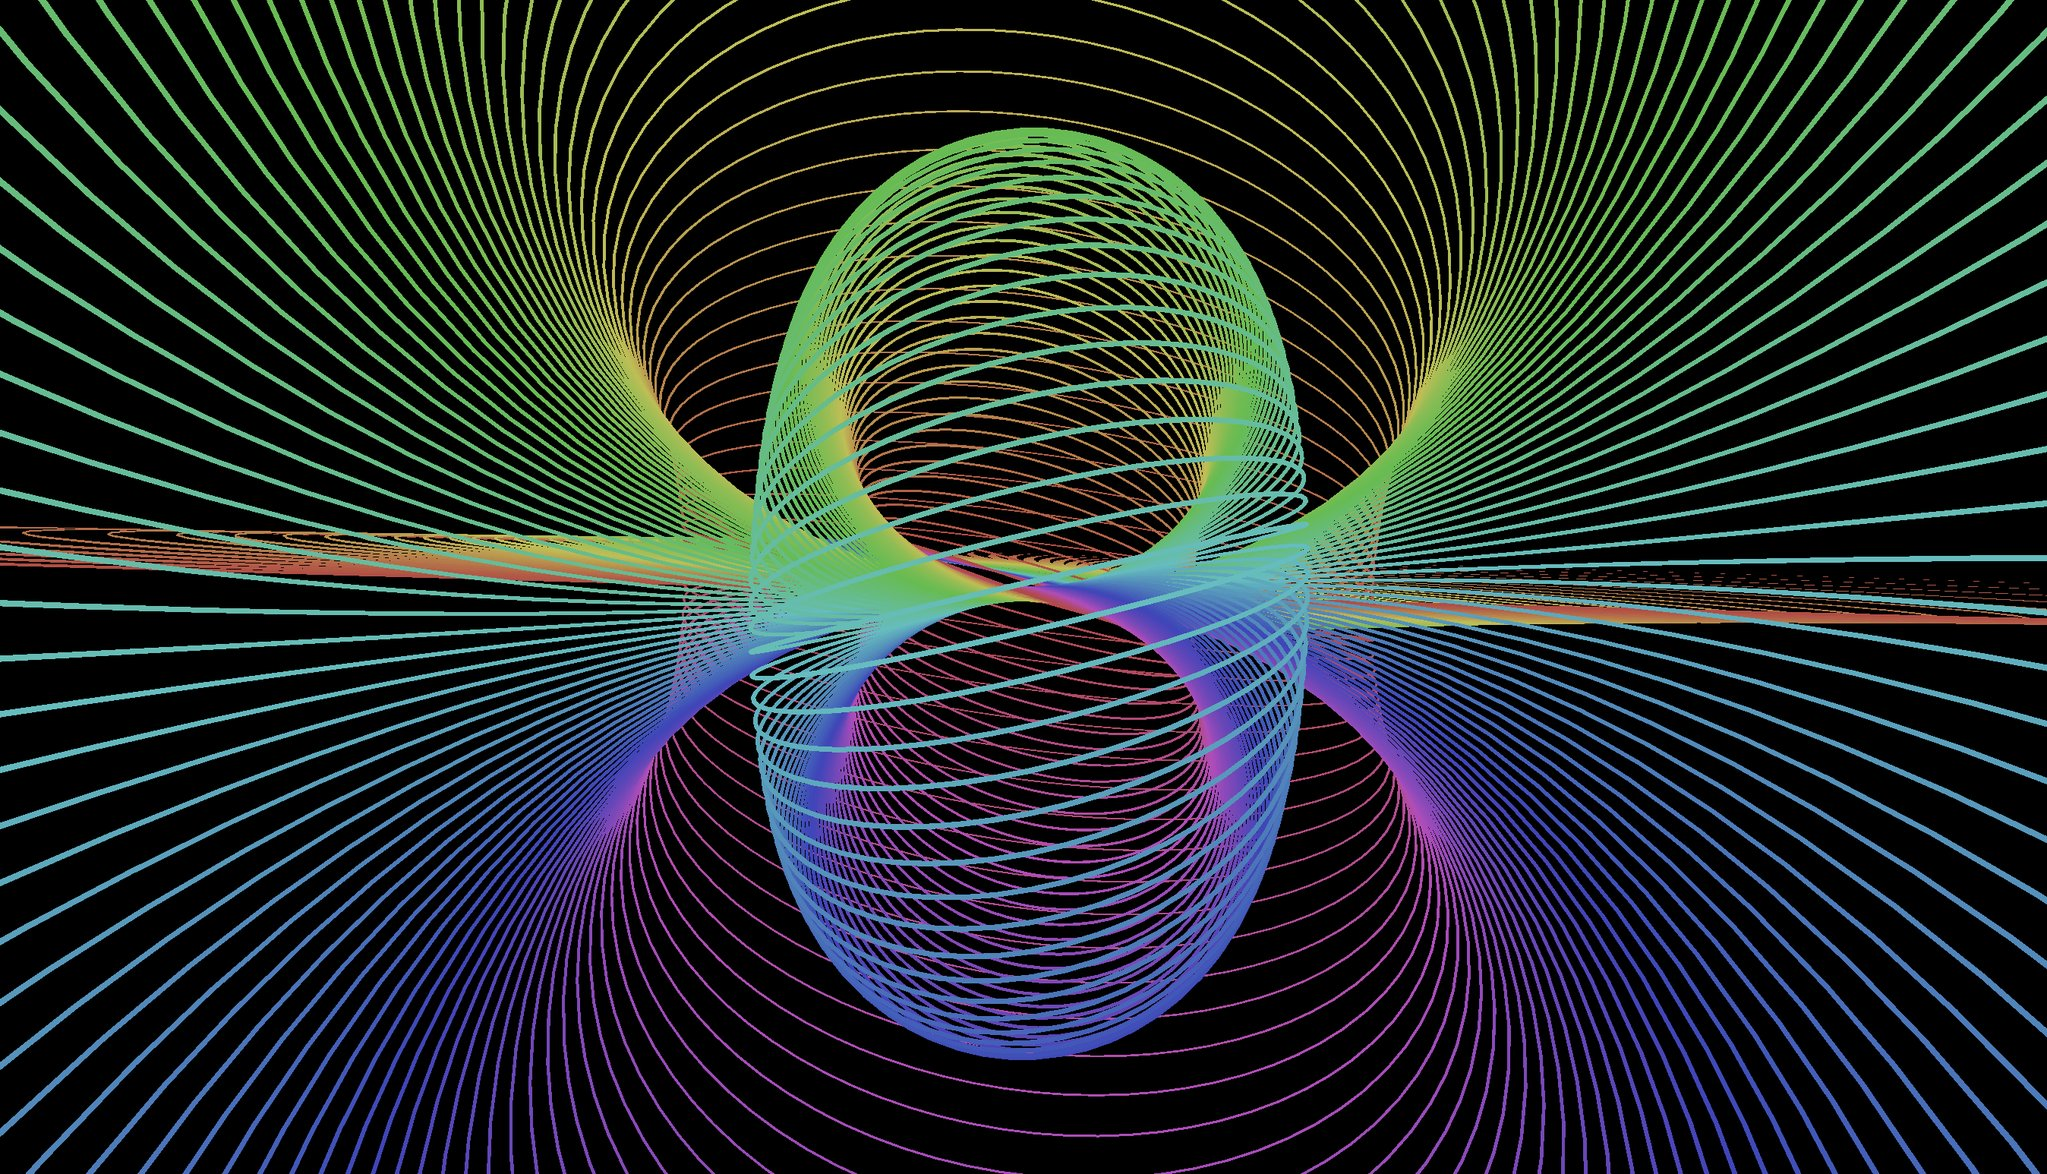
\includegraphics[scale=0.4]{hopf-2.jpeg}}
  \caption{Розшарування Хопфа}
\end{figure}
\begin{lstlisting}
var fiber = new THREE.Curve(),
    color = sphericalCoords.color;

fiber.getPoint = function(t) {
    var eta = sphericalCoords.eta,
        phi = sphericalCoords.phi,
        theta = 2 * Math.PI * t;
    var x1 = Math.cos(phi+theta) * Math.sin(eta/2),
        x2 = Math.sin(phi+theta) * Math.sin(eta/2),
        x3 = Math.cos(phi-theta) * Math.cos(eta/2),
        x4 = Math.sin(phi-theta) * Math.cos(eta/2);
    var m = mag([x1,x2,x3]),
        r = Math.sqrt((1-x4)/(1+x4));
        return new THREE.Vector3(r*x1/m,r*x2/m, r*x3/m);
    };
\end{lstlisting}
\end{definition}

\subsubsection*{Гомотопічна інтерпретація}
Can we reason about spheres without a metric? Yes!
But can we do this in a constructive way? Also yes.

\subsubsection{Розшарування Хопфа}
\begin{example} ($S^3$ Hopf Fiber).
Вперше розшарування Хопфа трьовимірної сфери було формалізовано Джильямом Брунері.
Тут дається його модифікована версія.
\begin{lstlisting}
rot: (x : S1) -> Path S1 x x = split
    base -> loop1
    loop @ i -> constSquare S1 base loop1 @ i

mu : S1 -> equiv S1 S1 = split
    base -> idEquiv S1
    loop @ i -> equivPath S1 S1 (idEquiv S1)
                (idEquiv S1) (<j> \(x : S1) -> rot x @ j) @ i

H : S2 -> U = split
    north -> S1
    south -> S1
    merid x @ i -> ua S1 S1 (mu x) @ i

total : U = (c : S2) * H c
\end{lstlisting}
\end{example}

\begin{definition} (H-space).
H-space over a carrier $A$ is a tuple
$$
H_A=
\begin{cases}
A : U\\
e : A\\
\mu : A \rightarrow A \rightarrow A\\
\beta : (a:A) \rightarrow \Sigma (\mu(e,a)=a) (\mu(a,e)=a)
\end{cases}
$$.
\end{definition}

\begin{theorem} (Hopf Fibrations).
There are fiber bundles: 
$(S^0,S^1,p,S^1)$,
$(S^1,S^3,p,S^2)$,
$(S^3,S^7,p,S^4)$,
$(S^7,S^{15},p,S^8)$.
\end{theorem}

\begin{definition} (Hopf Invariant).
Let $\phi: S^{2n-1} \rightarrow S^{n}$ a continuous map.
Then homotopy pushout (cofiber) of $\phi$ is
$cofib(\phi) = S^{n} \bigcup_\phi \mathbb{D}^{2n}$ has
ordinary cohomology
$$
H^{k}(cofib(\phi),\mathbb{Z})=
\begin{cases}
\mathbb{Z}\ for\ k=n,2n \\[2ex]
0\ otherwise
\end{cases}
$$
\end{definition}

Hence for $\alpha,\beta$ generators of the cohomology groups in
degree $n$ and $2n$, respectively, there exists an integer $h(\phi)$
that expresses the {\bf cup product} square of $\alpha$
as a multiple of $\beta$ --- $\alpha\sqcup\alpha=h(\phi)\cdot\beta$.
This integer $h(\phi)$ is called Hopf invariant of $\phi$.

\begin{theorem} (Adams, Atiyah).
Hopf Fibrations are only maps that have Hopf invariant $1$.
\end{theorem}

\subsection{Теорія гомологій}
\section{Диференціальна геометрія}
\subsection{V-многовиди}
\subsection{G-структури}
\subsection{H-простори}


